\documentclass[12pt,a4paper]{article}
\usepackage[a4paper,total={160mm,250mm}]{geometry}
\usepackage[utf8]{inputenc}
\usepackage{ngerman}
\usepackage{amsmath}
\usepackage{amsthm}
\usepackage{amsfonts}
\usepackage{amssymb}
\usepackage{amscd}
\usepackage{graphicx}
\usepackage{enumerate}
\usepackage{color}
\usepackage{mathtools}
\usepackage[ruled,vlined]{algorithm2e}
\usepackage{subcaption}

\pagestyle{empty}

\begin{document}
	\section*{Was ist Raytracing?}
	Raytracing bezeichnet eine Methode zur Generierung von realistischen 3D Bildern.
	Dabei kommen unter Anderem Reflexions- und Brechungsgesetze aus der Physik zur Anwendung.
	Vorallem aber beruht die Technik auf der Vektorgeometrie wie man sie am Gymnasium unterrichtet.
	Die Idee ist folgende: Wir verteilen einige Objekte (Kugeln, Würfel, etc.) im dreidimensionalen Raum.
	Wir nennen dies die Szene.
	Nun stellt man irgendwo eine Kamera auf.
	Vor der Kamera stellen wir uns eine rechteckige Fläche, die Bildebene, vor.
	Auf die Bildebene zeichnen wir nun die dahinter liegende Szene wie folgt:
	Ausgehend von der Kamera senden wir einen Strahl aus, der die Bildebene durchstösst und dann womöglich auf ein Objekt unserer Szene trifft.
	Trifft der Strahl zum Beispiel auf ein rotes Dreieck, so wird der Durchstosspunkt auf der Bildebene rot eingefärbt.
	Danach senden wir einen weiteren Strahl von der Kamera durch einen anderen Punkt auf der Bildebene und färben den Durchstosspunkt entsprechend ein.
	Wir wiederholen dies bis die ganze Bildebene eingefärbt ist.
	Das so auf der Bildebene generierte Abbild der Szene ist der Output unseres Programms.
	Diese Methode ein Bild zu generieren heisst Raytracing, denn man verfolgt den Strahl.
	\begin{figure}[h!]
		\centering
		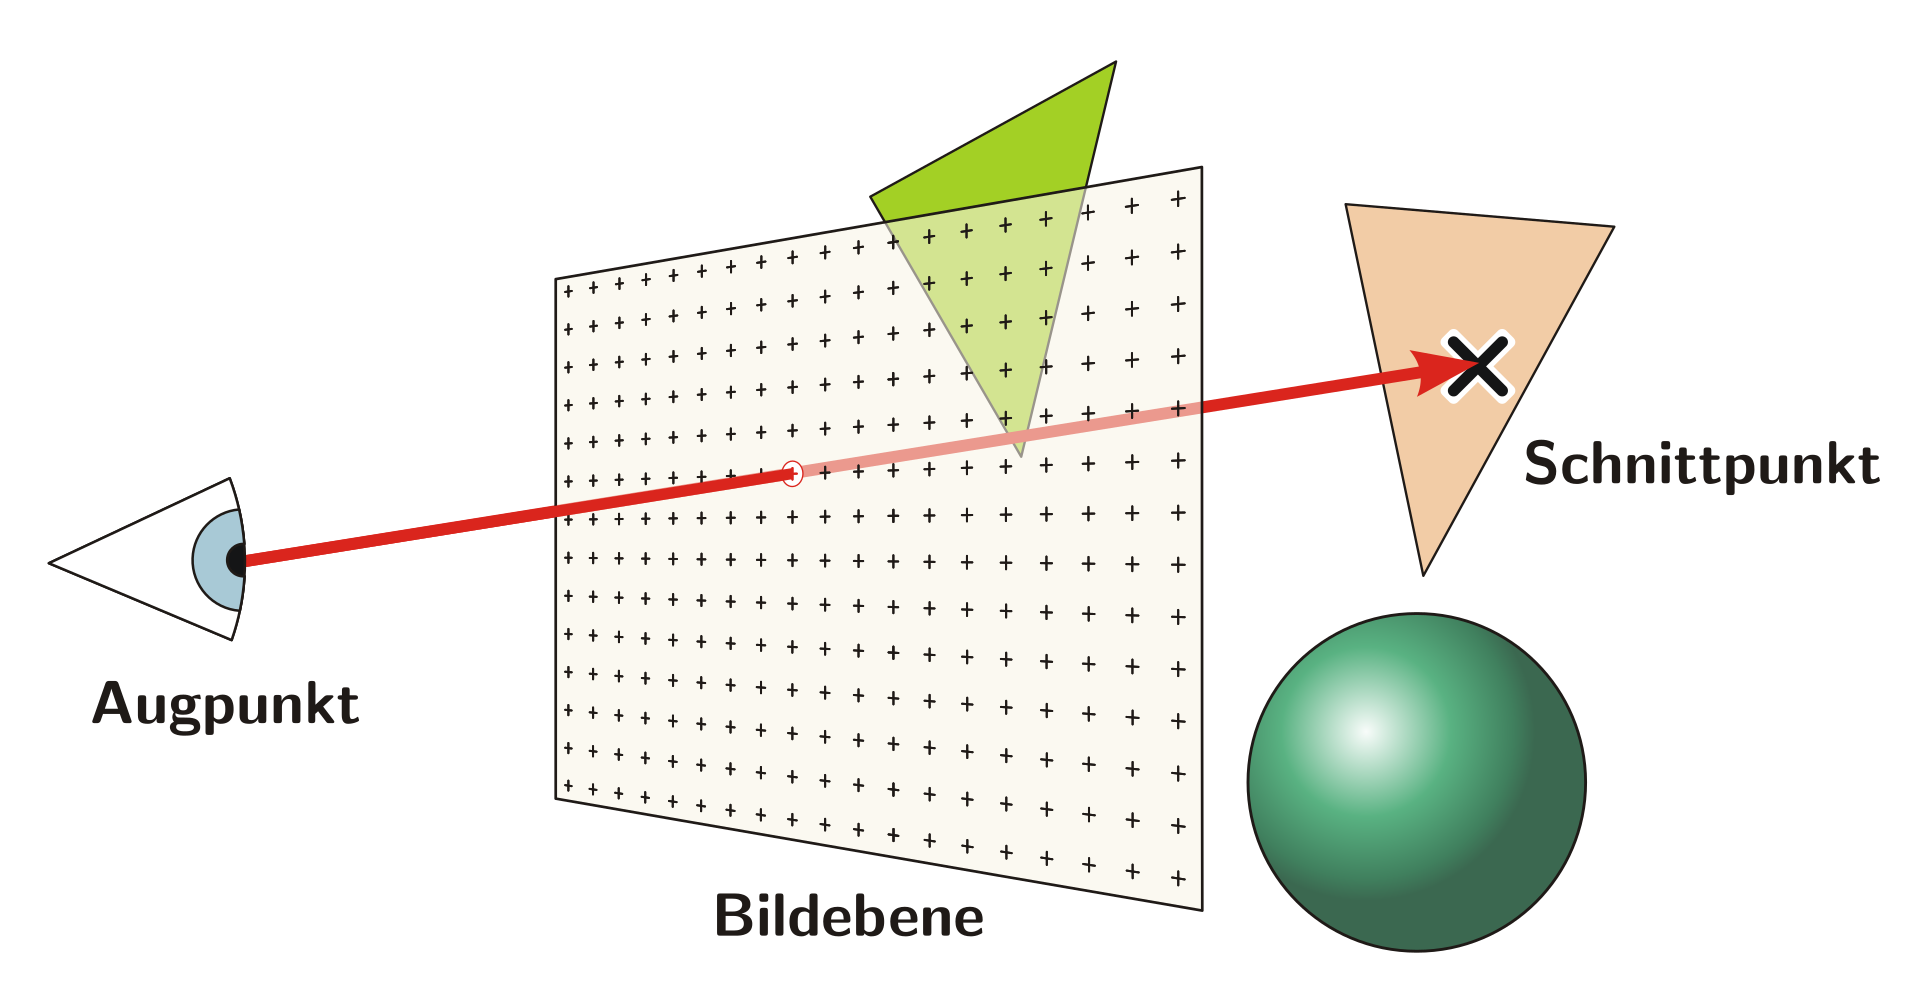
\includegraphics[width=\textwidth]{images/raytracing.png}
		\caption{Raytracing: Es werden Strahlen ausgesendet und deren Schnittpunkte mit Objekten ermittelt. In diesem Fall wir der Durchstosspunkt auf der Bildebene in der Farbe des roten Dreiecks gefärbt.}
		\label{fig:raytracing}
	\end{figure}

	\section*{Worum geht es im Folgenden?}
	Wir wollen nun unser eigenes Raytracing-Programm in Python programmieren.
	Genauer gesagt ist der Raytracing-Algorithmus im Kern schon implementiert.
	Allerdings kennt diese Implementierung noch keine Objekte wie Kugeln, Würfel, Ebenen und so weiter.
	Hier kommen Sie als Leser ins Spiel.
	Sie werden unter Anleitung diese fehlenden Teile ergänzen.
	Es geht darum dem Raytracing-Programm zu sagen, was zum Beispiel eine Kugel ist, wie man deren Schnittpunkt mit einem Strahl berechnet und vieles mehr.
	Am Ende werden wir Bilder wie in Abbildung~\ref{fig:goal} generieren können.
	\begin{figure}[h!]
		\centering
		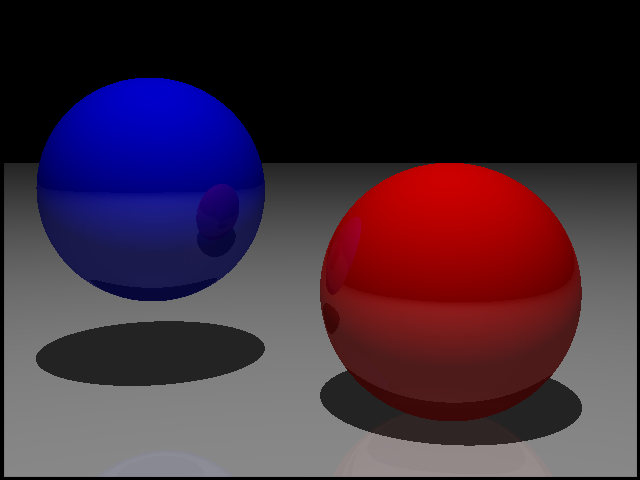
\includegraphics[width=0.75\textwidth]{images/image.png}
		\caption{Dieses Bild wurde mit unserem Raytracing-Programm generiert.}
		\label{fig:goal}
	\end{figure}

	\section*{Das erste Bild}
	
\end{document}
